\section{blockciphers}
\begin{frame}
	\frametitle{Blockciphers}
	blockciphers encrypt plaintext of a fixed length (64 bit and 128 bit are quite common)
	\vspace{1cm}
		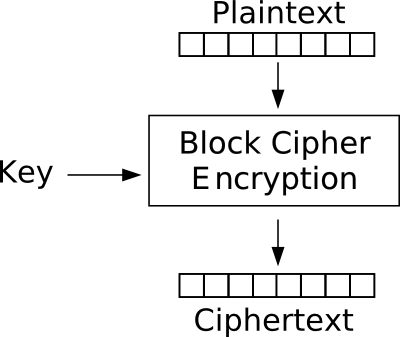
\includegraphics[width=4.5cm,height=3.5cm]{Encryption}
		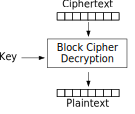
\includegraphics[width=4.5cm,height=3.5cm]{Decryption}
\end{frame}

\begin{frame}
\frametitle{structures of blockciphers}
	\begin{itemize}
		\item rounds
		\item feistel-network
		\item substitution-perumation-network
	\end{itemize}
\end{frame}


% ----
\begin{frame}
\frametitle{feistel-network}
	$L_{i+1} = R_i $ \\
	$R_{i+1} = L_i \oplus f(R_i, K_i)$
\end{frame}

% ----
